\documentclass[conference]{IEEEtran}
\IEEEoverridecommandlockouts
% The preceding line is only needed to identify funding in the first footnote. If that is unneeded, please comment it out.
\usepackage{cite}
\usepackage{amsmath,amssymb,amsfonts}
\usepackage{graphicx}
\usepackage{textcomp}
\def\BibTeX{{\rm B\kern-.05em{\sc i\kern-.025em b}\kern-.08em
    T\kern-.1667em\lower.7ex\hbox{E}\kern-.125emX}}
\begin{document}

\title{THE1\\
}

\author{\IEEEauthorblockN{Esref Ozturk}
\IEEEauthorblockA{\textit{CENG} \\
\textit{METU}\\
Ankara, Turkey \\
esrefozturk93@gmail.com}
}

\maketitle


\section{Introduction}
This report includes the discussions about CENG499 Machine Learning THE1 Homework \\

\section{Discussion}

\subsection{Effect of the Bias}

Accuracies with and without biases can be seen on the following table: \\

\begin{tabular}{l*{6}{c}r}
eta  & Accuracy(without bias) & Accuracy(with bias) \\
\hline
3e-4 & 0.4 & 0.48 \\
1e-3 & 0.57 & 0.58 \\
1e-1 & 0.65 & 0.79 \\
\end{tabular} \\

As it can be seen, bias increases the accuracy.

\subsection{Feature Scaling Technique}

Min-Max scaling technique is used for scaling each of the 8 features to 0-1 range. Using min-max scaling, all different range features are scaled to the same range. Luckily there was no feature that has the same max and min so min-max scaling were used.

\subsection{Effects of the Different Learning Rates}

Following table shows accuracy scores for different iteration counts: \\

\begin{tabular}{l*{6}{c}r}
eta  & 1000 & 10000 & 100000 \\
\hline
3e-4 & 0.37 & 0.48 & 0.61 \\
1e-3 & 0.37 & 0.58 & 0.73 \\
1e-1 & 0.73 & 0.79 & 0.79 \\
\end{tabular} \\

As iteration count increases, the gap between learning rates are decreasing. Small learning rates are causing the accuracy to increase very slowly. If we want to use small learning rates, we should increase the iteration count.

\subsection{Suggestion for a Better Learning Rate}

Using cross validation better learning rate can be selected. Also learning rate should be considered together with iteration count since for bigger iteration counts, smaller learning rates are enough.

\subsection{When to Stop Updates}

When to stop updates can be determined using cross validation. Iteration count can be parameterized for cross validation.

\subsection{Plots}

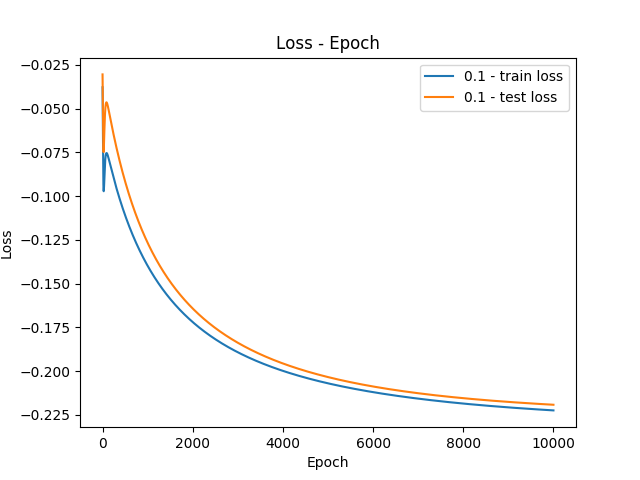
\includegraphics[width=0.5\textwidth]{loss.png}
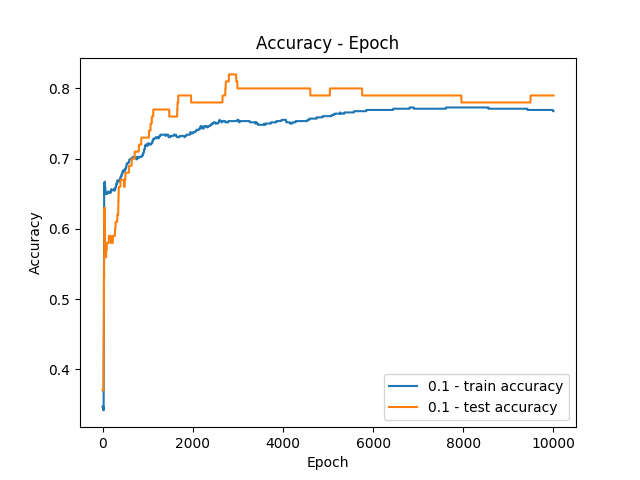
\includegraphics[width=0.5\textwidth]{accuracy.png}

\section{Conclusion}
Since the dataset  was consisting of independent variables, logistic regression was very handy at analyzing it.

\end{document}
